% !TeX root = skripta-konstitutivni-vztahy.tex
% !TeX lastmodified = 2018-10-10

\section{Teorie viskoelasticity}

\subsection{Co znamená pojem viskoelasticita?}
Viskozita – vlastnost kapaliny (tekutiny) – známe z hydromechaniky

Elasticita – vlastnost tuhé látky (tělesa) – známe z pružnosti a pevnosti

Viskoelasticita – spojení vlastností tekutiny a tuhé látky do společného konstitutivního modelu. Elastická látka i viskózní tekutina pak mohou být chápány jako jeho zvláštní případy.

\subsection{Podstata viskoelastického chování}
Materiál (každý) je v procesu zatěžování uveden do nerovnovážného stavu, kdy změny v rozmístění atomů naruší silovou rovnováhu. Je-li silová rovnováha obnovena velmi rychle (doba pro její dosažení je zanedbatelná), pak se odezva na zatížení jeví jako okamžitá a časově nezávislá (elastický materiál).

Není-li doba potřebná pro dosažení rovnovážného stavu zanedbatelná, pak se odezva materiálu jeví závislá na čase a materiál považujeme za viskoelastický. Po zatížení se nachází ve stavu termodynamicky nerovnovážném a rovnovážného stavu dosahuje teoreticky až za nekonečně dlouhou dobu.

\subsection{Osnova teorie lineární viskoelasticity}
\begin{enumerate}
	\item Vysvětlení základních pojmů
	\item Analogie mezi mechanikou kapalin a těles
	\item Základní vztahy lineární viskoelasticity 
	\item Popis chování viskoelastických látek pomocí nejjednodušších reologických modelů na základě jejich diferenciálních rovnic
	\begin{itemize}
		\item při statickém zatěžování
		\item při dynamickém (harmonickém) zatěžování
	\end{itemize}
	\item Využití teorie lineární viskoelasticity v MKP -- zadávání parametrů viskoelastických konstitutivních modelů v ANSYSu
\end{enumerate}

\subsection{Předpoklady lineární viskoelasticity}
\begin{itemize}
	\item Materiál je izotropní
	\item Jsou splněny podmínky linearity, především malé deformace (přetvoření do 1\%)
\end{itemize}

(pro velká časově závislá vratná přetvoření je třeba použít modely visko-hyperelastické)

\subsection{Analogie mechaniky těles a hydromechaniky}
Mechanika těles:
Cauchyho rovnice rovnováhy:
\begin{align}
	\frac{\partial \sigma_x}{\partial x} +
	\frac{\partial \tau_{yx}}{\partial y} +
	\frac{\partial \tau_{zx}}{\partial z} + o_x = 0\\
	\frac{\partial \tau_{xy}}{\partial x} +
	\frac{\partial \sigma_y}{\partial y} +
	\frac{\partial \tau_{zy}}{\partial z} + o_y = 0\\
	\frac{\partial \tau_{xz}}{\partial x} +
	\frac{\partial \tau_{yz}}{\partial y} +
	\frac{\partial \sigma_x}{\partial z} + o_z = 0
\end{align}
\begin{equation}
	T_\sigma = \left( \begin{matrix}
		\sigma_x & \tau_{xy} & \tau_{xz}\\
		\tau_{yx} & \sigma_y & \tau_{yz}\\
		\tau_{zx} & \tau_{zy} & \sigma_z
	\end{matrix} \right)
\end{equation}

\begin{equation}
	\vec{o} = \vec{A} \rho
\end{equation}

Machanika kapalin -- Eulerova rovnice hydrostatiky
\begin{align}
	A_x - \frac{1}{\rho} \frac{\partial p}{\partial x} = 0\\
	A_y - \frac{1}{\rho} \frac{\partial p}{\partial y} = 0\\
	A_z - \frac{1}{\rho} \frac{\partial p}{\partial z} = 0
\end{align}

Kontrolní otázka:
Zkuste zapsat v maticovém tvaru tenzor napětí pro ideální kapalinu
\subsection{Tvar tenzoru napětí pro ideální kapalinu}
\begin{itemize}
	\item Všechna normálová napětí záporná a~stejně velká -- důsledek Pascalova zákona
	\item Smyková napětí nulová -- důsledek nulové viskozity
\end{itemize}
\begin{equation}
T_\sigma = \left( \begin{matrix}
-p & 0 & 0\\
0 & -p & 0\\
0 & 0 & -p
\end{matrix} \right)
\end{equation}

\subsection{Analogie konstitutivních parametrů}
Mechanika těles
\begin{itemize}
	\item modul pružnosti v~tahu $E\:[Pa]$
	\item Poissonovo číslo $\mu\:[-]$
	\item Lamého konstanta $\lambda\:[Pa]$
	\item modul pružnosti ve smyku $G\:[Pa]$
	\begin{equation}
	\tau = G \gamma
	\end{equation}
	\item objemový modul pružnosti $K\:[Pa]$
	\begin{equation}
	K = \frac{\sigma_z}{e} = \frac{\frac{\sigma_x + \sigma_y + \sigma_z}{3}}{\frac{\Delta V}{V}}
	\end{equation}
\end{itemize}

Machanika kapalin
\begin{itemize}
	\item modul objemové stlačitelnosti $\varepsilon$
	\begin{equation}
		\varepsilon = -V \frac{\Delta p}{\Delta V}\:[Pa]
	\end{equation}
	\item dynamická viskozita $\eta$
	\begin{equation}
		\tau = \eta \frac{\diff c}{\diff n} = \eta \dot{\gamma}
	\end{equation}
\end{itemize}

Jaký je vztah mezi gradientem rychlosti v~kapalině a~rychlostí úhlové deformace tuhé látky?

Protože elastické vlastnosti izotropního materiálu jsou popsány dvěma nezávislými elastickými konstantami $G$ a~$K$, ostatní jsou závislé.
Pro společný popis je třeba vyjádřit Hookův zákon pomocí $G$ a~$K$. viz \ref{sec:hookeuv-zakon}

\subsection{Způsoby popisu lineárně viskoelastického chování látek}
\begin{enumerate}
	\item Spojitý popis pomocí konvolučních integrálů (matematicky komplikovanější, vysvětlení je založeno na zobecnění reologických modelů uvedených dále).
	\item Zjednodušený popis pomocí reologických modelů, tvořených kombinací základních reologických prvků.
\end{enumerate}

\subsection{Reologické modely viskoelastického chování}
\begin{itemize}
	\item Musíme odděleně modelovat tvarovou (konstanty $G$, $\eta$) a objemovou (konstanty $K$, $\kappa$) změnu.
	\item Chování reologických modelů si ukážeme na deviátorové části tenzoru napětí a~přetvoření, tedy na tvarové změně (závislosti smykového napětí a~zkosu). Stejným způsobem se modeluje i objemová změna.
	\item Pro obě části lze použít stejného typu modelu, ale objemová změna se často modeluje jako čistě elastická, protože u~objemové změny je její viskózní složka podstatně méně významná.
\end{itemize}

\begin{figure}[H]
	\centering
	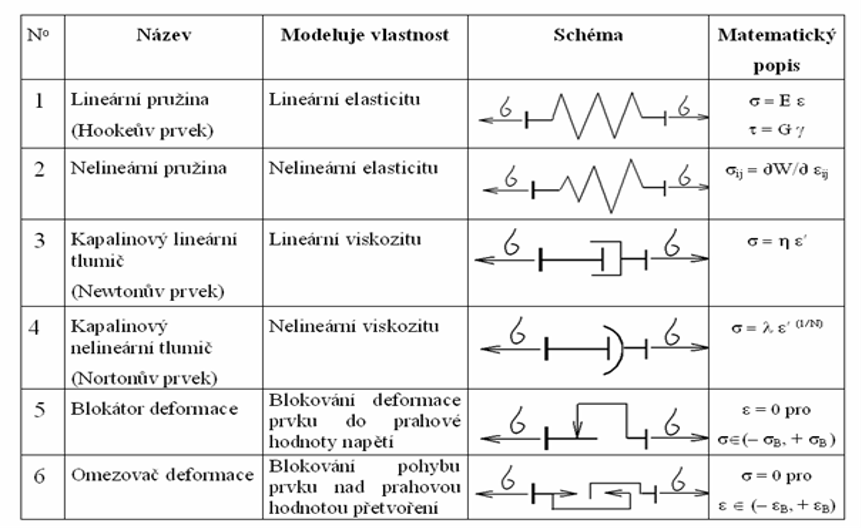
\includegraphics[width=0.8\linewidth]{Obrazky/prvky-reologickych-modelu}
	\caption{Základní prvky reologických modelů }
	\label{fig:prvky-reologickych-modelu}
\end{figure}

\subsection{Nejjednodušší reologické modely viskoelastické látky}
\subsubsection{Maxwellův model}
\begin{figure}[H]
	\centering
	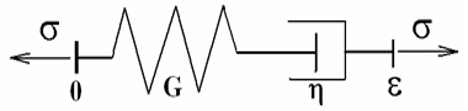
\includegraphics[height=2cm]{maxwelluv-model}
	\caption{Maxwellův model}
	\label{fig:maxwelluv-model}
\end{figure}

Diferenciální rovince
\begin{equation}
	\frac{\diff \sigma}{\diff t} + \frac{\sigma}{\frac{\eta}{G}} = G \frac{\diff \varepsilon}{\diff t},
\end{equation}
kde $\tau = \frac{\eta}{G}\:[s]$ je časová konstanta přechodového děje.

Pro konstantní silové zatížení $\sigma_0$, tedy creep, dostaneme řešením diferenciální rovnice odezvu
\begin{equation}
	\eta(t) = \frac{\sigma_0}{G} + \frac{\sigma_0}{\eta} t.
\end{equation}
Deformace tedy roste lineárně s~časem, tzv. volný creep.

Pro konstantní deformační zatížení $\varepsilon_0$ dostaneme řešením diferenciální rovnice exponenciální odezvu pro relaxaci napětí
\begin{equation}
	\sigma(t) = G \varepsilon_0 \exp^{-\frac{t}{\tau}}
\end{equation}

\subsubsection{Kelvinův-Voigtův model}
\begin{figure}[H]
	\centering
	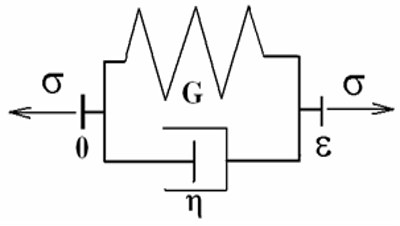
\includegraphics[height=2cm]{kelvinuv-voigtuv-model}
	\caption{Kelvinův-Voigtův model}
	\label{fig:kelvinuv-voigtuv-model}
\end{figure}

Diferenciální rovince
\begin{equation}
	\frac{\diff \varepsilon}{\diff t} + \frac{\varepsilon}{\frac{\eta}{G}} = \frac{\sigma}{\eta},
\end{equation}
kde $\tau = \frac{\eta}{G}\:[s]$ je časová konstanta přechodového děje.

Pro konstantní silové zatížení $\sigma_0$ dostaneme řešením diferenciální rovnice creepovou odezvu
\begin{equation}
	\varepsilon(t) = \frac{\sigma_0}{G} \left(1 - \exp^{-\frac{t}{\tau}} \right)
\end{equation}

Deformace se tedy blíží exponenciálně k asymptotické hodnotě -- vázaný creep.
Skokové změny deformace nelze dosáhnout (nutno $\sigma \rightarrow \infty$).

\begin{figure}[H]
	\centering
	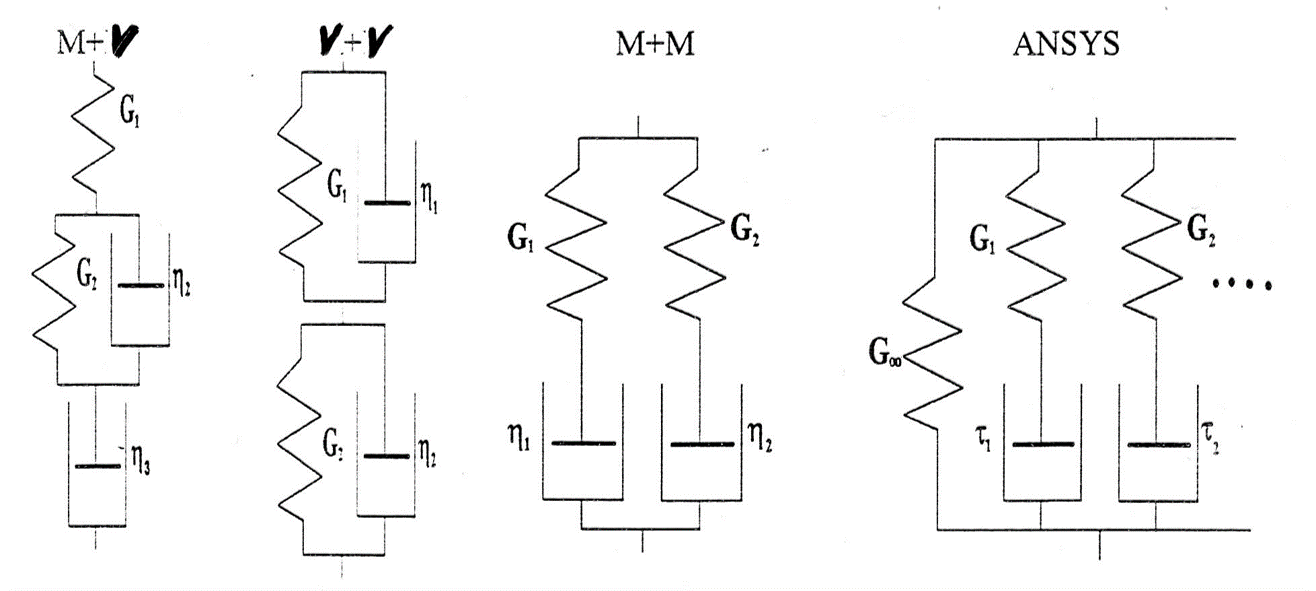
\includegraphics[width=0.75\linewidth]{slozitejsi-reologicke-modely}
	\caption{Příklady složitějších reologických modelů viskoelastického chování}
	\label{fig:slozitejsi-reologicke-modely}
\end{figure}

\begin{figure}[H]
	\centering
	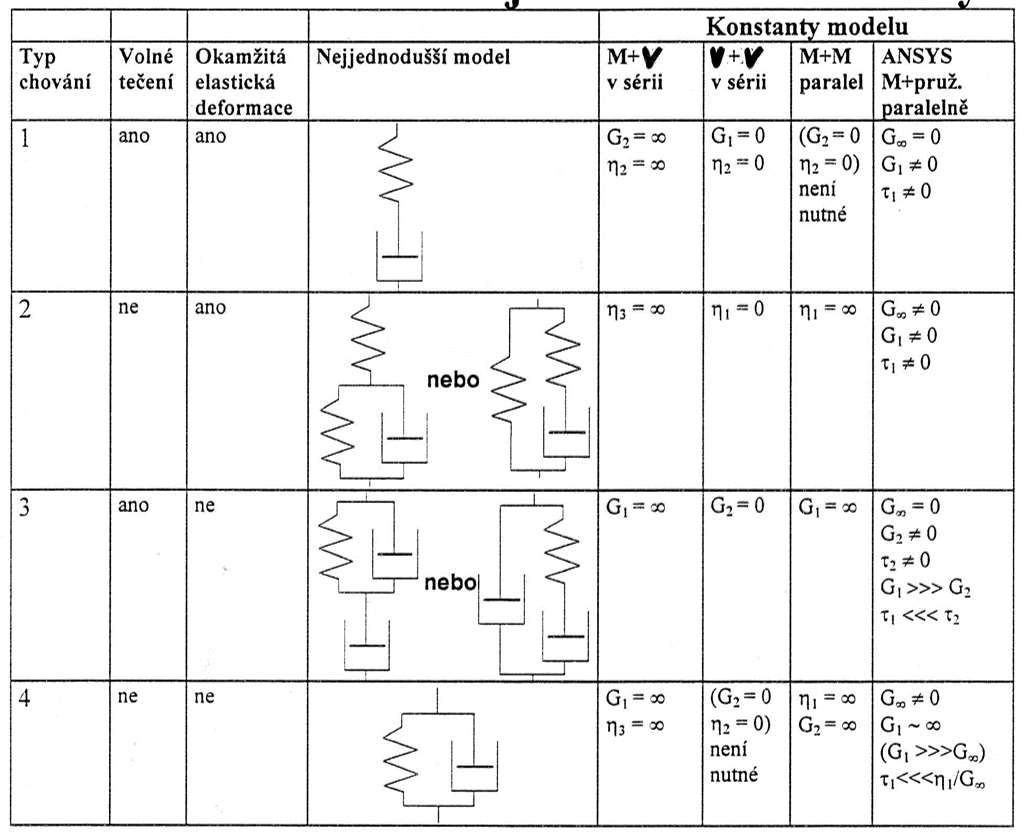
\includegraphics[width=0.75\linewidth]{reologicke-modely}
	\caption{Reologické modely pro základní typy viskoelastického chování}
	\label{fig:reologicke-modely}
\end{figure}

\subsubsection{Standard linear solid}
\begin{figure}[H]
	\centering
	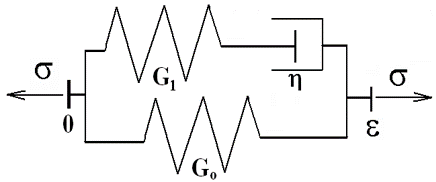
\includegraphics[height=2cm]{standard-linear-solid}
	\caption{Standard linear solid}
	\label{fig:standard-linear-solid}
\end{figure}

Diferenciální rovnice
\begin{equation}
	\sigma + \tau_\varepsilon \frac{\diff \sigma}{\diff t} = G_0 \left(\varepsilon + \tau_\sigma \frac{\diff \varepsilon}{\diff t}\right)
\end{equation}
kde relaxační doba při konstantní deformaci je $\tau_\varepsilon = \frac{\eta}{G_1}$ a~retardační doba při konstantním napětí je $\tau_{12}\sigma = \frac{\eta}{G_0} \left(1 + \frac{G_0}{G_1}\right)$

\begin{figure}[H]
	\centering
	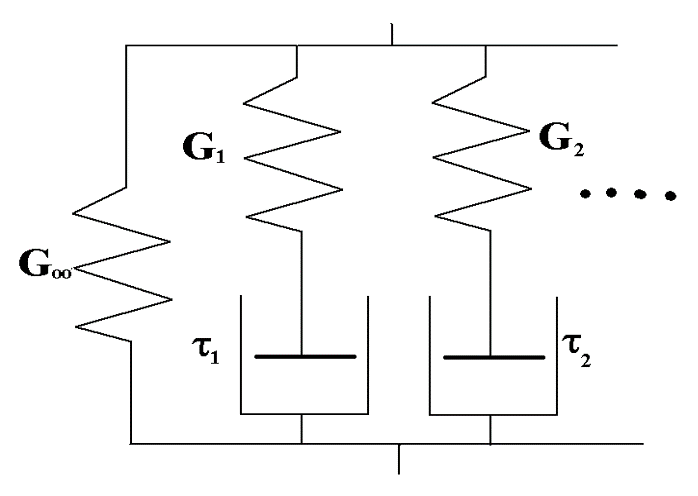
\includegraphics[width=0.3\linewidth]{zobecneny-maxwelluv-model}
	\caption{Zobecněný Maxwellův model v~ANSYSu}
	\label{fig:zobecneny-maxwelluv-model}
\end{figure}

\begin{figure}[H]
	\centering
	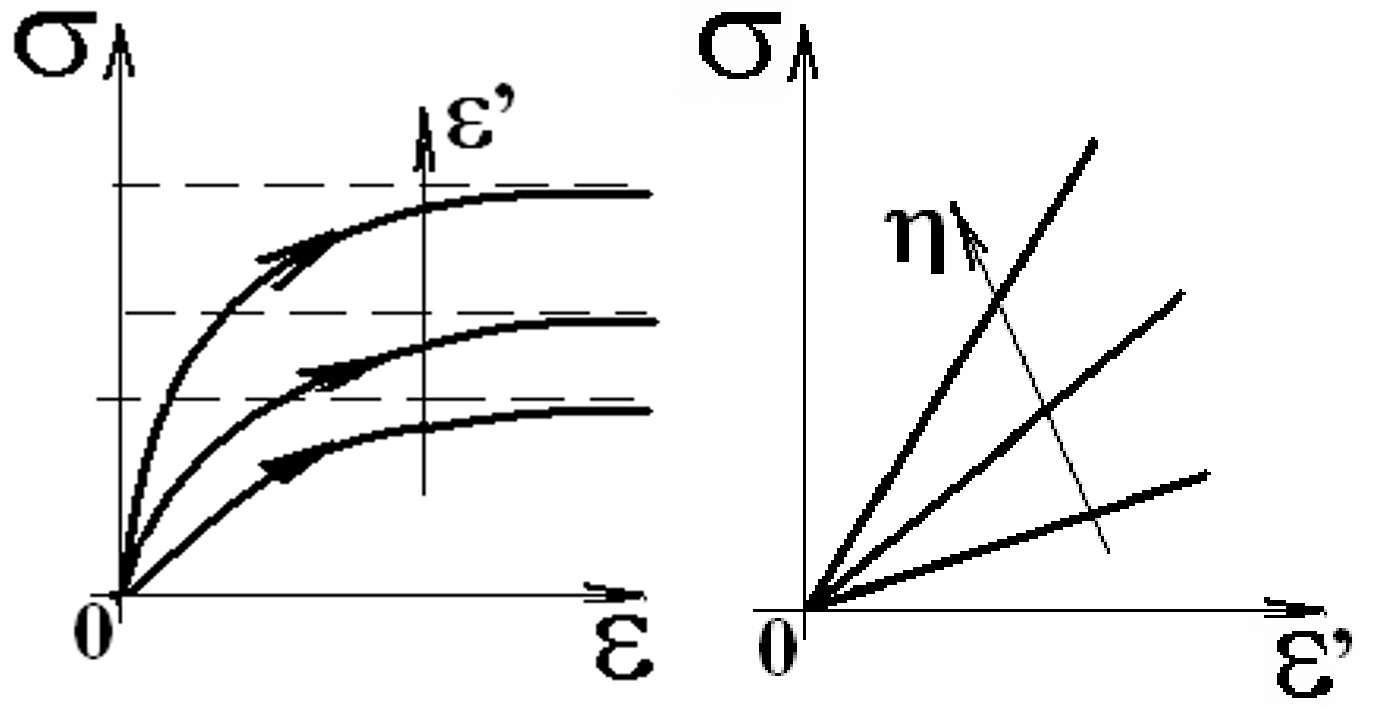
\includegraphics[width=0.5\linewidth]{tahova-zkouska-maxwellova-modelu}
	\caption{Deformačně-napěťové závislosti (tahová zkouška) Maxwellova modelu}
	\label{fig:tahova-zkouska-maxwellova-modelu}
\end{figure}

\begin{figure}[H]
	\centering
	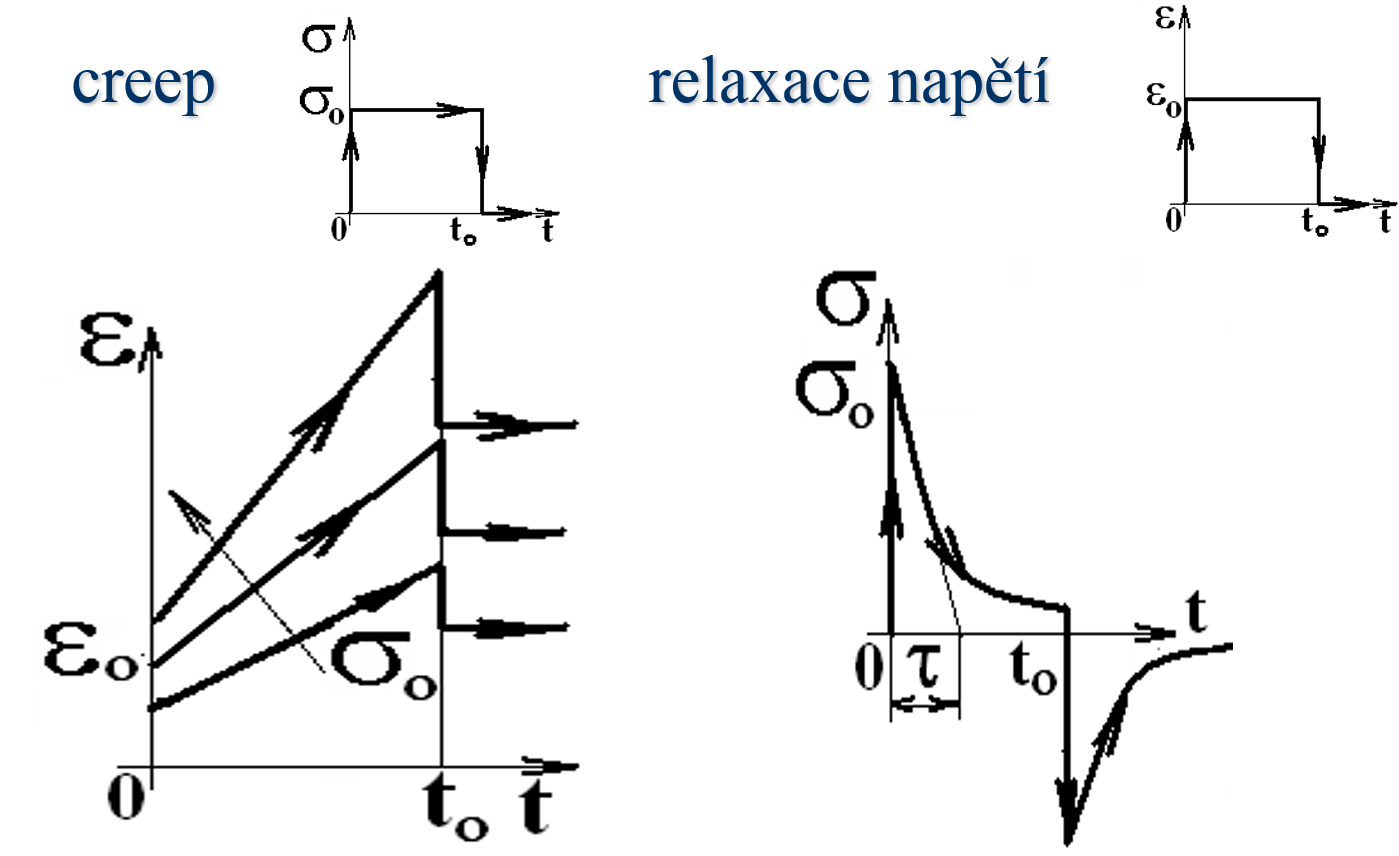
\includegraphics[width=0.5\linewidth]{odezva-maxwellova-modelu}
	\caption{Odezva Maxwellova modelu při statickém zatížení}
	\label{fig:odezva-maxwellova-modelu}
\end{figure}

\subsection{Znázornění harmonického zatěžování v~komplexní rovině pro Kelvinův-Voigtův model s~řízenou deformací}
Umožňuje vyjádření komplexního modulu pružnosti
Odezva na harmonický průběh napětí $\varepsilon = \varepsilon_a \cos(\omega t)$
Deformace viskózního členu předbíhá deformaci o~$\frac{\pi}{2}$.

\begin{figure}[H]
	\centering
	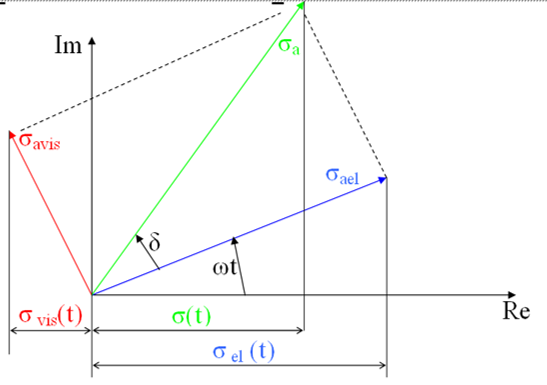
\includegraphics[width=0.5\linewidth]{komplexni-rovina-kelvinova-voigtova-modelu}
	\caption{Kelvinův-Voightův model v~komplexní rovnice}
	\label{fig:komplexni-rovina-kelvinova-voigtova-modelu}
\end{figure}

$\delta$ -- fázový posuv

Ztrátový faktor $\tan(\delta)$ je nepřímo úměrný úhlové frekvenci zatěžování
\begin{equation}
	\tan(\delta) = \frac{G}{\eta \omega}
\end{equation}

Z~grafu lze vyjádřit přetvoření
\begin{equation}
	\sigma(t) = \sigma_a \cos(\omega t + \delta),
\end{equation}
kde amplituda $\varepsilon_a$ je dána
\begin{equation}
	\sigma_a = \sqrt{\left( G \varepsilon_a \right)^2 + \left( \eta \omega \varepsilon_a \right)^2}.
\end{equation}

\subsection{Znázornění harmonického zatěžování v~komplexní rovině pro Maxwellův model s~řízeným napětím}
Umožňuje vyjádření komplexního modulu pružnosti
Odezva na harmonický průběh napětí $\sigma = \sigma_a \cos(\omega t)$
Deformace viskózního členu ze zpožďuje za napětím o~$\frac{\pi}{2}$.

\begin{figure}[H]
	\centering
	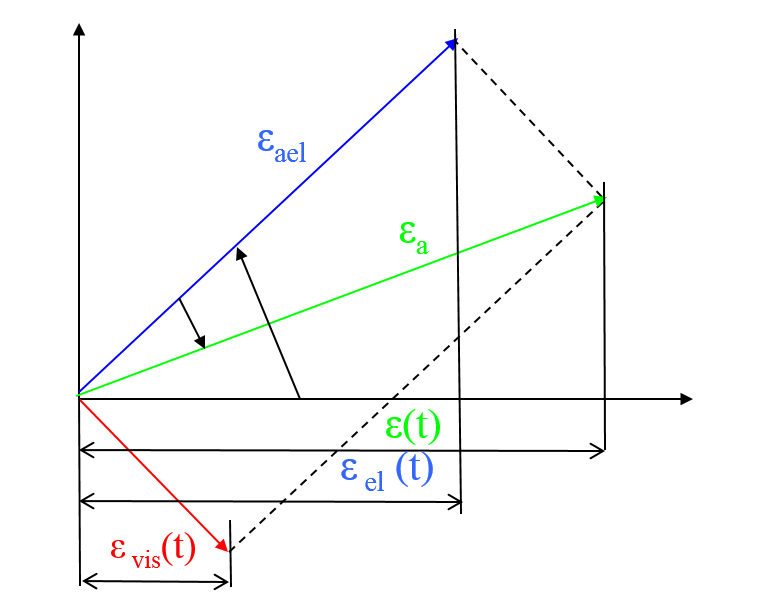
\includegraphics[width=0.5\linewidth]{komplexni-rovina-maxwellova-modelu}
	\caption{Maxwellův model v~komplexní rovnice}
	\label{fig:komplexni-rovina-maxwellova-modelu}
\end{figure}

$\delta$ -- fázový posuv

Ztrátový faktor $\tan(\delta)$ je nepřímo úměrný úhlové frekvenci zatěžování
\begin{equation}
	\tan(\delta) = \frac{G}{\eta \omega}
\end{equation}

Z~grafu lze vyjádřit přetvoření
\begin{equation}
	\varepsilon(t) = \varepsilon_a \cos(\omega t - \delta),
\end{equation}
kde amplituda $\varepsilon_a$ je dána
\begin{equation}
	\varepsilon_a = \sqrt{\left(\frac{\sigma_a}{G}\right)^2 + \left(\frac{\sigma_a}{\eta \omega}\right)^2}.
\end{equation}

\subsection{Závislost viskoelasticity na teplotě}
Popisuje se na základě experimentů\footnote{M.L. Williams, R.F. Landel, and J.D. Ferry. "The Temperature Dependence of Relaxation Mechanisms in Amorphous Polymers and Other Glass-forming Liquids". Journal of the American Chemical Society. Vol. 77. 3701-3706. 1955}.

\begin{figure}[H]
	\centering
	\caption{Křivka}
	\label{fig:zavislost-viskoelasticity-na-teplote}
	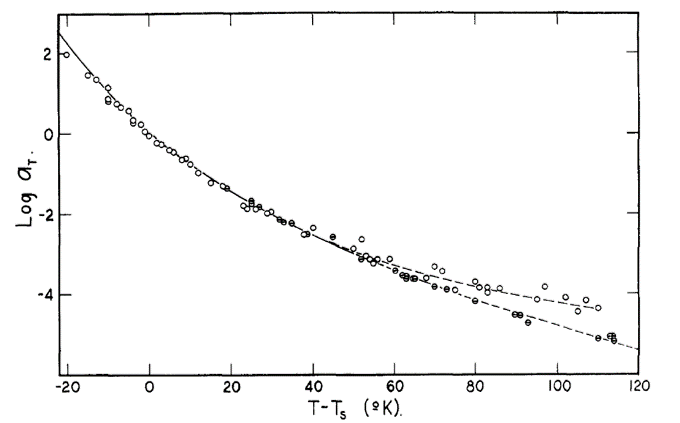
\includegraphics[width=0.5\linewidth]{zavislost-viskoelasticity-na-teplote}
\end{figure}

$a_T = \frac{\tau_T}{\tau_T^\text{ref}}$\\
$T_s = T_\text{ref}$ -- referenční teplota

\subsection{Popis závislosti viskoelasticity na teplotě}
Na základě uvedené závislosti mezi teplotou a~změnou viskozity (časové konstanty), která je přibližně stejná pro většinu polymerů i~jiných látek, formulovali \textsc{Wiliams}, \textsc{Landal} a~\textsc{Ferry} rovnici ve tvaru:
\begin{equation}\label{eq:williams-landal-ferry}
	\log_{10} a_T = 	\frac{c_1 (T - T_\text{ref})}{c_2 + T - T_\text{ref}},
\end{equation}
kde
\begin{description}
	\item[$T$] je aktuální teplota,
	\item[$T_\text{ref}$] je referenční teplota,
	\item[{$C_1 [\si{\per\kelvin}], C_2 [\si{\kelvin}]$}] jsou materiálové parametry.
\end{description}

$T_\text{ref}$ se volí obvykle cca $\SI{50}{\celsius}$ nad teplotou skelného přechodu $T_g$ a~vztah platí v~intervalu ($T_g$ ; $T_g +100$) $[\si{\kelvin}]$.

Vztah (\ref{eq:williams-landal-ferry}) odpovídá popisu v~menu ANSYSu. V~nápovědě ANSYSu (a~zřejmě i~reálně naprogramován) je vztah
\begin{equation}\label{eq:williams-landal-ferry-ansys}
\log_{10} a_T = \frac{-c_1 (T - T_\text{ref})}{c_2 + T - T_\text{ref}},
\end{equation}
s~mínusem (a~další konstantou, která zůstává nulová) a~používá (zřejmě omylem) $\ln$ místo $\log$. 

\subsection{Praktické využití modelů lineární viskoelasticity}
\begin{itemize}
	\item Při měření a~používání elastických konstant je nutné brát v~úvahu rychlost zatěžování (resp. rychlost deformace -- běžná tahová zkouška má rychlost přetvoření řádu $10^{-2} s^{-1}$).
	\item Při výpočtech je nutno pracovat odděleně s~kulovou a~deviátorovou složkou tenzorů $T_\sigma$ a~$T_\varepsilon$, neboť mají různé časové konstanty, tedy různý podíl elastické a~viskózní složky.
	\item \framebox[\linewidth]{I~jednoosá napjatost (při tahové zkoušce) se skládá ze složky kulové a~deviátorové!}
	\item Viskoelastický model vysvětluje
	\begin{itemize}
		\item tečení (volný i~vázaný creep)
		\item relaxaci napětí
		\item hysterezi (bez zbytkové trvalé deformace)
	\end{itemize}
	\item Z~chování materiálu při určitém typu zatěžování (např. skoková změna napětí při krípové zkoušce) a~odpovídající modelové představy lze předpovědět chování  při jiných typech zatěžování (např. při dynamickém namáhání).
	\item Možnost numerického řešení viskoelastického chování pomocí MKP -- např. v~ANSYSu zobecněný Maxwellův model použitý v modelech viskoelastického chování tzv. “Prony series” nebo v prvcích VISCO88 (rovinný) a~VISCO89 (prostorový).
	\item Neznáme-li objemovou viskozitu, nejreálnějším předpokladem je čistě elastické chování v~objemové složce, tedy objemová (druhá) viskozita blížící se nekonečnu.
	\item Neznáme-li objemový modul pružnosti a~víme pouze, že materiál je téměř nestlačitelný, volíme objemový modul pružnosti o~několik řádů vyšší než smykový. Chyba způsobená neznalostí konkrétní hodnoty objemového modulu pružnosti je pak obvykle zanedbatelná.
\end{itemize}
